\documentclass{article}

\usepackage[final]{nips_2017}
\usepackage[utf8]{inputenc} % allow utf-8 input
\usepackage[T1]{fontenc}    % use 8-bit T1 fonts
\usepackage{hyperref}       % hyperlinks
\usepackage{url}            % simple URL typesetting
\usepackage{booktabs}       % professional-quality tables
\usepackage{amsfonts}       % blackboard math symbols
\usepackage{nicefrac}       % compact symbols for 1/2, etc.
\usepackage{microtype}      % microtypography
\usepackage{bm}             % bold in math
\usepackage{graphicx}       % images
\usepackage{algorithm}      % algorithm
\usepackage[noend]{algpseudocode} % algorithm
\usepackage{caption}        % captionof
\usepackage{array}          % thick column hline
\usepackage{booktabs}       % table style
\usepackage{pbox}           % table line break
\usepackage{subcaption}     % multiple figuresx
\usepackage{tikz}
\usetikzlibrary{positioning, fit, arrows.meta, shapes}
\usepackage{amsmath}


\title{Biomedical Named Entity Recognition with Attention}
\hypersetup{
    colorlinks = true,
}
\makeatletter
\def\BState{\State\hskip-\ALG@thistlm}
\makeatother
\floatname{algorithm}{Procedure}
\renewcommand{\algorithmicrequire}{\textbf{Input:}}
\renewcommand{\algorithmicensure}{\textbf{Output:}}

\newcolumntype{?}{!{\vrule width 3pt}}

\author{
  Hao Wu\\
  University of Illinois at Urbana-Champaign\\
  Urbana, IL \\
  \texttt{haow11@illinois.edu} \\
  \And
  Peilun Zhang \\
  University of Illinois at Urbana-Champaign\\
  Urbana, IL \\
  \texttt{peilunz2@illinois.edu} \\
}


\DeclareMathOperator*{\argmax}{argmax}
\begin{document}

\maketitle

\begin{abstract}
Biomedical named entity recognition (BioNER) is a specific sequence to sequence (seq2seq) task. Given a sequence of words, the goal is to obtain the best or most possible sequential labels, such as genes, chemicals and diseases. Currently, most sequence labeling methods heavily rely on Bi-directional Long Short-Term Memory-Conditional Random Field (BiLSTM-CRF) models. Transformer that utilizes attention mechanism shows promising results in handling seq2seq problems, which provides us with insights to modify the BiLSTM-CRF models to utilize attention mechanism to conduct BioNER. We propose an Attention-CRF model to selectively encode the representation of sequential words, and recognize the sequence of labels. We evaluate the performance of our learning framework on 15 BioNER datasets compared with state-of-the-art BioNER frameworks and baselines. We further compare and analyze the time complexity of BiLSTM-CRF and Attention-CRF as seq2seq models.
\end{abstract}
%%%%%%%%%%% 
% Introduction
%%%%%%%%%%% 
\section{Introduction}
With more and more literature produced in the biomedical area, building an efficient toolkit to automatically extract knowledge from documents becomes increasingly necessary. To handle this requirement, BioNER plays an important role that aims to recognize biomedical entities, such as genes, chemicals, and diseases without too many human efforts. Besides, it is also beneficial for many downstream applications, like relation extraction, event detection and document summarization. 

% Current work on BioNER, handcraft and nn based for feature encoding
Generally, BioNER is regarded as a sequence labeling task, which means we should assign the best label sequence to the input word sequence. Traditional methods often require handcrafted features to locate specific entity types. For instance, we can frequently see the suffix '-ase' more in proteins than diseases~\citep{habibi2017deep}. However, generating such amount of domain-specific features for BioNER system requires domain knowledge and cannot be directly adapted to recognize new entity types. Rather than manually designing entity-specific features, recent works mainly focus on developing an automatic learning algorithm to extract latent features of sequential words to feed a conditional random field (CRF)~\citep{lafferty2001conditional} layer to predict the output label sequence. \citet{habibi2017deep} followed the suggestion from \citet{lample2016neural} and proposed BiLSTM-CRF model to predict the label sequence with completely agnostic knowledge to every type of the entity. This neural network model only requires golden dataset with entity labels and pre-trained word embedding from large, domain-specific corpus (e.g. all PubMed abstracts). \citet{wang2018cross} improves the ability of BiLSTM-CRF network with multi-task learning by sharing BiLSTM layers .

% Development on feature encoding
Currently, with the fast development of attention mechanism~(\citet{vaswani2017attention},~\citet{bah2015},~\citet{LuongPM15}), researchers work on building new model architecture for feature encoding that eschews recurrence but instead relies on only the attention mechanism to encode the sequential information about input corpus. \citet{vaswani2017attention} proposed one novel sequence transduction model, called Transformer, based solely on attention mechanism. \citet{lee2019biobert} applied a pre-trained biomedical language representation model based on BERT architecture~\citep{devlin2018bert} which performs well in three representative biomedical text mining tasks, including BioNER. 

In this paper, we combine the idea of BiLSTM-CRF~\citep{habibi2017deep} model and self-attention mechanism~\citep{vaswani2017attention}, by replacing feature encoding layer of BiLSTM with a self attention layer~\citep{vaswani2017attention} to represent character level information and word level information. Outputs of those layers are then still fed to a CRF layer to do the final label sequence predictions. We call it Attention-CRF model. This method completely eschews the sequential computation, and only needs to parameterize the attention assigned on each unit (word or character) to encode the unit information. We evaluate and compare the performance of Attention-CRF with other 4 neural network architecture in 15 benchmark biomedical dataset used by \citep{crichton2017neural}.
%%%%%%%%%%% 
% Background
%%%%%%%%%%% 
\section{Background}

\subsection{Problem definition of Name Entity Recognition (NER)}

 Given a word sequence $\textbf{w} = \{w_1, w_2, ..., w_n\}$, we should assign the best label sequence $\textbf{l} = \{l_1, l_2, ..., l_n\}, l_i \in L$ to each word separately, where L includes every possible labels according to IOBES schemes (see \ref{exp:iobes}). For example, if we are given a sentence "Selegiline - induced postural hypotension...", the best label sequence should be like "S-Chemical O O B-Disease E-Disease...". Because in this sentence, "selegiline" is a kind of chemical and "postural hypotension" is a disease, whereas other words are out of chunks.

\subsection{Long Short-Term Memory (LSTM)}
\begin{figure}[h]
\newcommand{\empt}[2]{$#1_{#2}$}
\resizebox{\linewidth}{!}{
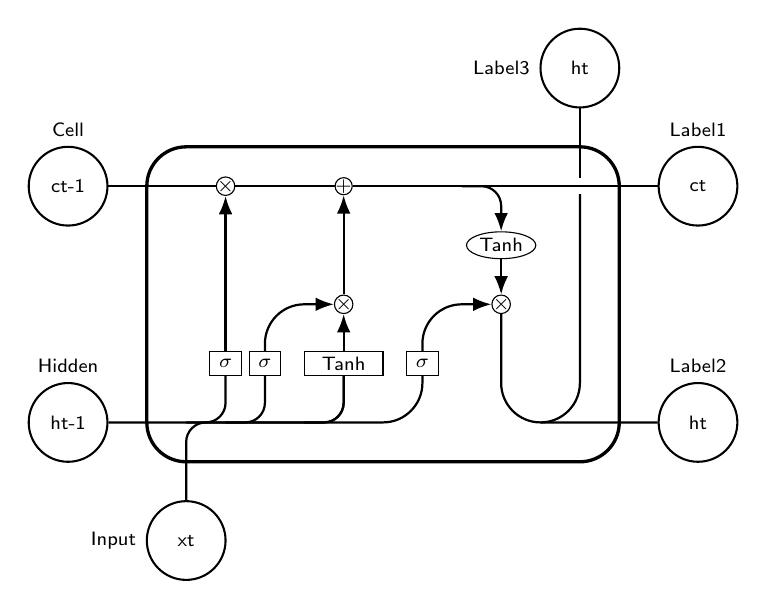
\begin{tikzpicture}[
    % GLOBAL CFG
    font=\sf \scriptsize,
    >=LaTeX,
    % Styles
    cell/.style={% For the main box
        rectangle, 
        rounded corners=5mm, 
        draw,
        very thick,
        },
    operator/.style={%For operators like +  and  x
        circle,
        draw,
        inner sep=-0.5pt,
        minimum height =.2cm,
        },
    function/.style={%For functions
        ellipse,
        draw,
        inner sep=1pt
        },
    ct/.style={% For external inputs and outputs
        circle,
        draw,
        line width = .75pt,
        minimum width=1cm,
        inner sep=1pt,
        },
    gt/.style={% For internal inputs
        rectangle,
        draw,
        minimum width=4mm,
        minimum height=3mm,
        inner sep=1pt
        },
    mylabel/.style={% something new that I have learned
        font=\scriptsize\sffamily
        },
    ArrowC1/.style={% Arrows with rounded corners
        rounded corners=.25cm,
        thick,
        },
    ArrowC2/.style={% Arrows with big rounded corners
        rounded corners=.5cm,
        thick,
        },
    ]

%Start drawing the thing...    
    % Draw the cell: 
    \node [cell, minimum height =4cm, minimum width=6cm] at (0,0){} ;

    % Draw inputs named ibox#
    \node [gt] (ibox1) at (-2,-0.75) {$\sigma$};
    \node [gt] (ibox2) at (-1.5,-0.75) {$\sigma$};
    \node [gt, minimum width=1cm] (ibox3) at (-0.5,-0.75) {Tanh};
    \node [gt] (ibox4) at (0.5,-0.75) {$\sigma$};

   % Draw opérators   named mux# , add# and func#
    \node [operator] (mux1) at (-2,1.5) {$\times$};
    \node [operator] (add1) at (-0.5,1.5) {+};
    \node [operator] (mux2) at (-0.5,0) {$\times$};
    \node [operator] (mux3) at (1.5,0) {$\times$};
    \node [function] (func1) at (1.5,0.75) {Tanh};

    % Draw External inputs? named as basis c,h,x
    \node[ct, label={[mylabel]Cell}] (c) at (-4,1.5) {\empt{c}{t-1}};
    \node[ct, label={[mylabel]Hidden}] (h) at (-4,-1.5) {\empt{h}{t-1}};
    \node[ct, label={[mylabel]left:Input}] (x) at (-2.5,-3) {\empt{x}{t}};

    % Draw External outputs? named as basis c2,h2,x2
    \node[ct, label={[mylabel]Label1}] (c2) at (4,1.5) {\empt{c}{t}};
    \node[ct, label={[mylabel]Label2}] (h2) at (4,-1.5) {\empt{h}{t}};
    \node[ct, label={[mylabel]left:Label3}] (x2) at (2.5,3) {\empt{h}{t}};

% Start connecting all.
    %Intersections and displacements are used. 
    % Drawing arrows    
    \draw [ArrowC1] (c) -- (mux1) -- (add1) -- (c2);

    % Inputs
    \draw [ArrowC2] (h) -| (ibox4);
    \draw [ArrowC1] (h -| ibox1)++(-0.5,0) -| (ibox1); 
    \draw [ArrowC1] (h -| ibox2)++(-0.5,0) -| (ibox2);
    \draw [ArrowC1] (h -| ibox3)++(-0.5,0) -| (ibox3);
    \draw [ArrowC1] (x) -- (x |- h)-| (ibox3);

    % Internal
    \draw [->, ArrowC2] (ibox1) -- (mux1);
    \draw [->, ArrowC2] (ibox2) |- (mux2);
    \draw [->, ArrowC2] (ibox3) -- (mux2);
    \draw [->, ArrowC2] (ibox4) |- (mux3);
    \draw [->, ArrowC2] (mux2) -- (add1);
    \draw [->, ArrowC1] (add1 -| func1)++(-0.5,0) -| (func1);
    \draw [->, ArrowC2] (func1) -- (mux3);

    %Outputs
    \draw [-, ArrowC2] (mux3) |- (h2);
    \draw (c2 -| x2) ++(0,-0.1) coordinate (i1);
    \draw [-, ArrowC2] (h2 -| x2)++(-0.5,0) -| (i1);
    \draw [-, ArrowC2] (i1)++(0,0.2) -- (x2);

\end{tikzpicture}
}
\caption{Architecture of Long Short-Term Memory Neural Network.}
\label{lstm_arch}
\end{figure}
Recurrent neural networks (RNNs) are a kind of neural networks that conduct operations upon sequential data. The input to a RNN is a sequence of vectors ($x_1, x_2, ..., x_t$), where each vector $x_i$ is a representation of an element in the input sequence. The output generated by the network is another sequence ($h_1, h_2, ..., h_t$) that represents some information about sequence at each step, where each vector $h_i$ is a hidden state vector. Although RNNs can learn long dependencies, previous work has also found out that RNNs, in practice, appears to be biased towards the most recent inputs~\citep{bengio1994} because when training a RNN using back-propagation, the gradients can tend to zero or infinity due to the usages of numbers with finite precision.

Long short-term memory (LSTM) neural network is a designated type of RNN that aims to model dependencies between sequence elements~\citep{lstm1997}. Figure~\ref{lstm_arch} illustrates an architecture of LSTM neural network. At step $t$ of recurrent calculation, $c_t$ represents memory stored in cell, $h_t$ represents the output hidden state, $x_t$ is the input vector, $\sigma$ denotes element-wise sigmoid function, $tanh$ denotes element-wise hyperbolic tangent function, $+$ and $\times$ denotes element-wise summation and multiplication.  At step $t$ of the recurrent calculation, the inputs of the network are $x_t$, $c_\text{t-1}$, $h_\text{t-1}$ and the outputs of the network are $c_t$, $h_t$. Previous work~\citep{wang2018cross} uses the following implementation:
\begin{align*} 
i_t &= \sigma(W^ix_t + U^ih_{t-1} + b^i)\\
f_t &= \sigma(W^fx_t + U^fh_{t-1} + b^f)\\
o_t &= \sigma(W^ox_t + U^oh_{t-1} + b^o)\\
g_t &= tanh(W^gx_t + U^oh_{g-1} + b^g)\\
c_t &= f_t \odot c_{t-1} + i_t \odot g_t \\
h_t &= o_t \odot tanh(c_t)'
\end{align*}
where $i_t, f_t$ and $o_t$ are referred as input, forget, and output gates. Initially, $h_0$ and $c_0$ are zero vectors and the parameters to train are $W^j, U^j$ and $b^j$ for $j\in\{i,f,o,g\}$.

\subsection{Bi-directional Long Short-Term Memory (BiLSTM)}
LSTM model computes a sequence of hidden state vectors that represents the previous context of the sentence at each word. It is intutive that the subsequent context can also provide useful information.

Inspired by this idea, Bi-directional Long Short-Term Memory (BiLSTM) improves the LSTM model by feeding inputs twice with different directions, one in the original direction, the other in the reversed direction~\citep{bilstm}. Then, the outputs from each directions are aggregated together as the final output, which captures the dependencies from not only the previous elements but also the subsequent elements of the sequence.


\subsection{Bi-directional Long Short-Term Memory-Conditional Random Field (BiLSTM-CRF)}
A very simple tagging model can use the output hidden state vectors as features to make independent tagging decisions. However, a limitation of this strategy appears when the dependencies across the labels are very strong. NER is a typical example of such task because the grammatical structure has significant affects on the labels but the structure will not be modeled with independent assumptions. It is useful and important to model the dependencies across output labels. Previous work utilizes a conditional random field to conduct this task and has shown a promising result~\citep{lafferty2001conditional}. For an input sequence, $X$ = ($x_1, x_2, ..., x_n$), and output sequence $y$ = ($y_1, y_2, ..., y_n$), a score is defined as:\\
\begin{align*}
    s(X,y)= \sum_{i=0}^{n} A_{y_i, y_{i+1}} + \sum_{i=1}^{n} P_{i, y_i}
\end{align*}
where $n$ is the length of the sequence, $k$ is the number of distinct labels, $P$ is an $n \times k$ matrix of the output from the BiLSTM layer, $A_{i,j}$ is the transition probability from label $i$ to label $j$. There are two additional labels that represents \textit{start} and \textit{end} of the sequences and therefore A is a matrix with dimension $(k+2)\times(k+2)$.

The training process maximizes the log-probability of the correct label sequence: 
\begin{align*}
    log(p(y|X)) = s(X,y) - log(\sum_{\widetilde{y}\in Y_X} e^{(s(X, \widetilde{y})))}
\end{align*}
where $Y_X$ are defined as all possible label sequences for a input sequence $X$. During the prediction stage, the model predicts the output sequence by:

\begin{align*}
   y^* = \argmax_{\widetilde{y}\in Y_X} s(X, \widetilde{y})
\end{align*}
\subsection{Attention}
Inspired by the observations that certain alignment exists between the input sequence and output sequence, which means that each step of generating a token is greatly related to a certain part of the input sequence, attention mechanism aims to allow the model to refer back to the input sequence~\citep{young2018recent}. An attention network keeps a set of hidden state representations that scale with the size of the input sequence. The model performs selection over the representations to allow the model to maintain a variable-length memory~\citep{structatten}. 

For input sequence $(x_1, x_2, ..., x_n)$, let $z$ be a categorical latent variable with sample space \{1, 2, ..., n\} that represents the selection among input, and let $q$ be a query. The mechanism aims to generate a context $c$ with the input sequence and a query, by accessing to a distribution $z \mathtt{\sim} p(z|x, q)$ that can be derived from applying softmax function to vectors of alignment scores, where it conditions $p$ on the input $x$ and a query $q$. Then, the context over a sequence is defined as:
\begin{align*}
    c = \mathbb{E}_{z \mathtt{\sim} p(z|x, q)} [f(x, z)]
\end{align*}
where $f(x, z)$ is a compatibility function. Two types of compatibility functions are majorly used, dot-product compatibility function~\citep{LuongPM15}~\citep{vaswani2017attention} and multi-layer perceptron compatibility function~\citep{bah2015}. 


%%%%%%%%%%% 
% Background
%%%%%%%%%%% 
\section{BioNER Model with Attention}
%%%%%%%%%%% 
% Experiment
%%%%%%%%%%% 
\section{Experiment}

\subsection{Dataset}
The datasets we use in this paper to evaluate the performance of BioNER models were introduced by \citet{crichton2017neural}. They provided 15 datasets focusing on biomedical name entity types. These datasets contain several entity types about biomedical and they are all publicly accessible. The details of datasets above are listed in Table~\ref{table:dataset}, including the name of datasets, name entity types, and entity counts.

Following the data splitting metrics of \citet{lample2016neural}, we separate the datasets into three sections: training section, development section , and test section. We use training section to optimize our neural networks, whose hyperparamters are tuned on development section. And the performance of the model will be evaluated in the test section. The training set will include most data items, around $70\%$ of all data items, and the development and test set will contain around $10\%$ and $20\%$ datasets respectively. The size of development section should not be too large, because it is used to tune the hyperparameters by many times of repeated experiments.

The sequence of labels is encoded by IOBES schemes. According this schemes, each word can be annotated with 5 kinds of label. The IOBES format is following IOB format (inside-outside-beginning). It is a tagging format for tagging tokens from sequences.

\begin{itemize}\label{exp:iobes}
    \item I: I- prefix indicates the tag is in the chunk
    \item O: O- prefix indicates the tag is outside a chunk
    \item B: B- prefix means the tag is the beginning the chunk and is followed by tags with same entity types
    \item E: E- prefix means the tag is the end of the chunk
    \item S: S- prefix indicates single tag of the chunk
\end{itemize}

\subsubsection{Dataset Benchmarks}

\begin{table}[]
\caption{The datasets and details of their annotations}
\label{table:dataset}
\resizebox{\columnwidth}{!}{
\begin{tabular}{|l|l|l|}
\hline
\textbf{Dataset} & \textbf{Entity Types} & \textbf{Entity Counts} \\ \hline
\textbf{AnatEM} & Anatomy NE & 13,701 \\ \hline
\textbf{BC2GM} & Gene/Protein NE & 24,583 \\ \hline
\textbf{BC4CHEMD} & Chemical NE & 84,310 \\ \hline
\textbf{BC5CDR} & Chemical, Disease NEs & \begin{tabular}[c]{@{}l@{}}Chemical: 15,935; \\ Disease: 12,852\end{tabular} \\ \hline
\textbf{BioNLP09} & Gene/Protein NE & 14963 \\ \hline
\textbf{BioNLP11EPI} & Gene/Protein NE & 15,811 \\ \hline
\textbf{BioNLP11ID} & 4 NEs & \begin{tabular}[c]{@{}l@{}}Gene/Protein: 6551; Organism: 3471;\\ Chemical: 973; Regulon-operon: 87\end{tabular} \\ \hline
\textbf{BioNLP13CG} & 16NEs & \begin{tabular}[c]{@{}l@{}}Gene/Protein: 7908; Cell: 3492;\\ Cancer: 2582; Chemical: 2270; \\ Multi-tissue structure: 857; Tissue: 587;  \\ Cellular component: 569; Organ: 421; \\ Organism substance: 283; \\ Pathological formation: 228; \\ Amino acid: 135; Organism: 1715;\\ Immaterial anatomical entity: 102; \\ Organism subdivision: 98; \\ Anatomical system: 41;\\ Developing anatomical structure: 35\end{tabular} \\ \hline
\textbf{BioNLP13GE} & Gene/Protein NE & 12,057 \\ \hline
\textbf{BioNLP13PC} & 4 NEs & \begin{tabular}[c]{@{}l@{}}Gene/Protein: 10,891; \\ Chemical: 2487; Complex: 1502; \\ Cellular component: 1013\end{tabular} \\ \hline
\textbf{CRAFT} & 6 NEs & \begin{tabular}[c]{@{}l@{}}SO: 18,974; Gene/Protein: 16,064;\\ Taxonomy: 6868; Chemical: 6053; \\ CL: 5495; GO-CC: 4180\end{tabular} \\ \hline
\textbf{Ex-PTM} & Gene/Protein NE & 4698 \\ \hline
\textbf{JNLPBA} & 5 NEs & \begin{tabular}[c]{@{}l@{}}Gene/Protein: 35,336; \\ DNA: 10,589; Cell Type: 8639;\\ Cell Line: 4330; RNA: 1069\end{tabular} \\ \hline
\textbf{Linnaeus} & Species NE & 4263 \\ \hline
\textbf{NCBI-Disease} & Disease NE & 6881 \\ \hline
\end{tabular}
}
\end{table}

\subsection{Pre-trained Word Embedding}
\citet{moen2013distributional} created a bunch of word vectors trained from the entire available biomedical scientific literature, a text corpus of over five billion words. It includes three separate data sources: (1) Abstracts form PubMed dataset (PubMed); (2)  Full-text documents from PubMed Central (PMC); (3) English Wikipedia dump (Wiki). 

\citet{habibi2017deep} studied the impact of different word embeddings trained from different combination of data sources listed above. They reported that the Wiki-PubMed-PMC embeddings achieve the best performance in all their evaluations. This dataset provides a set of word vectors with 200 dimensions induced on a combination of PubMed and PMC texts with texts extracted from a recent English Wikipedia dump \citep{moen2013distributional}. 

\subsection{Evaluation Metrics}
All evaluation results are conducted on each test dataset. \citet{wang2018cross} mentioned \textit{exact match} is one solution to evaluate the prediction, which means only that the predicted entity type and entity boundary are the same as the ground truth will be considered as "matched". After that, we calculate the precision, recall, micro-F1 and macro-F1 scores for each dataset independently to check the performance of each model on different dataset. Moreover, we also provide these metrics for each name entity to show the performance of each model on handling different entity types. We want to figure out whether each model is sensitive to the specific entity types. For example, if the entity count is small, the model will fail to capture the information about that entity type and give a bad result.

We compare the set of false positives (FPs) and false negatives (FNs) of the different BioNER methods (\citet{habibi2017deep}, \citet{wang2018cross}) for error analysis. Thus, in the result section, we will show the error samples of each model and the sequence of labels together.

\subsection{Baseline Methods}
In the experiment, we will compare our Attention-CRF model with 4 previous neural network models:
\begin{enumerate}
    \item Vanilla BiLSTM-CRF (VBC): A three layer BiLSTM-CRF architecture was employed by \citet{lample2016neural} and \citet{habibi2017deep}. They took the characters of each word in to the first BiLSTM layer to produce a character-level representation for this word. Then the character-level vector was concatenated with word embedding and fed into the second BiLSTM layer to produce label distribution. Finally, a CRF layer was added to maximize the log probability of label sequence.
    \item Single Task Model (STM): Compared with vanilla BiLSTM-CRF, \citet{wang2018cross} proposed STM to handle out-of-vocabulary (OOV) words. They still adopted three layer BiLSTM-CRF architecture but considered the character sequence of the input sentence rather than word as the input of the first BiLSTM layer.
    \item LM-LSTM-CRF (LLC):
    \item Tie or Break (ToB): \citet{shang2018learning} regarded the NER task as entity span detection and entity type prediction problem. It had no CRF layer and was reported being more efficient than BiLSTM-CRF models.
\end{enumerate}

\bibliographystyle{plainnat}
\bibliography{bib}
\end{document}
